
\documentclass[12pt]{article}
\usepackage[letterpaper,textwidth=5.5in,right=0.6in,textheight=9in,left=0.6in,top=0.7in,bottom=0.7in]{geometry}

\usepackage{amsmath,amssymb}
\usepackage{graphicx}

\begin{document}
	\noindent Xinshi Wang\\
	661975305\\
	hw03\\
	
	\noindent 1.\\
	\textbf{Proof:} Assume there exists $M_{P1}$ and $M_{P2}$ such that $M_{P1} \neq M_{P2}$. Consider one leaf node $v$ for tree $T$. Since $T$ has a perfect match, the parent vertex of $v$ denoted as $u$ could only have one childb(Otherwise some leaf vertices will not be saturated). Then we remove all the leaf vertices which gives us $\{e_1,e_2,...e_n\}$. We repeat this process untill we have no vertices. Since in every iteration the edges between the leaf vertices and parent vertices are unique, the set ${e_1,e_2,...,e_n}$ which is the set of edges in perfect match, is unique. Thus $M_{p1}$ must equal to $M_{p2}$.
	\hfill $\blacksquare$
	
	\noindent 2.\\
	\textbf{Proof:} Since the match $|M| = \dfrac{|V(G)|}{2}$, we know $M$ is a perfect match. We know $G$ has a perfect match $M$ iff $o(G-S) \leq |S|, \forall S \subseteq V(G)$ from the Tutte condition. In this case, $S$ is a single vertex $v$. Since graph G has a perfect match, $o(G-v) \leq 1$. There are two exhuastive cases, $o(G-v) = 0$ or $o(G-v) = 1$. If $o(G-v) = 0$, there are no odd componenets, which means all components are even. Thus we have $|V(G)|-1$(since we removed one vertex) being even. Since we know $|V(G)|$ is even, $|V(G)|-1$ must be odd, which forms a contradiction. Thus it must be the case $o(G-v) =1$, which means G has exactly one odd component.
	\hfill $\blacksquare$
	
	\noindent 3.\\
	\textbf{Proof:} We need to prove two statements. (1). $S$ is a vertex cover $\implies$ $\bar{S}$ is an independent set. (2). $\bar{S}$ is an independent set $\implies$ $S$ is a vertex cover.
	
	Let us first prove $S$ is a vertex cover $\implies$ $\bar{S}$ is an independent set. Let us assume that $\exists (u,v) \in E(\bar{S})$, then $\nexists (u,v) \in E(S)$ by the definition of a complement graph. Since $u \in V(S)$, $v \in V(S)$, and $\nexists (u,v) \in E(S)$, $S$ is not an vertex cover which leads to a contradiction. Thus $\forall u,v \in \bar{S}$, $\nexists (u,v) \in E(\bar{S})$. In other words, no vertices in $\bar{S}$ are connected. Thus $\bar{S}$ is an vertex cover.
	
	Let us next prove $\bar{S}$ is an independent set of graph $G = (V,E)$ $\implies$ $S$ is a vertex cover. If $\bar{S}$ is an independent set, then $\forall (u,v) \in E(G)$, at most one vertex is in $\bar{S}$ otherwise it is not an independent set. Therefore at least one vertex is in $S$. Therefore every pair of vertices has at least one endpoint in S, which implies $S$ is an vertex cover.
	
	\hfill $\blacksquare$
	
	\noindent 4. $|8| \leq |\text{vetex cover}| \leq 21$
	
	From the $Konig$ theorem, we know the cardinality of minimum vertex cover of G equals the cardinality of the maximum match of G. Thus minimum vertex cover = $|M| = 9 - 1$(one vertex is unsaturated). The maximum vertex cover is the the cardinality of the vertex set since all vertices must cover the edge set of G. 
	
		\hfill $\blacksquare$
	\newpage
	
	\noindent 5. $0<|M| \leq 12$.
	
	From the $Konig$ theorem, we know the cardinality of minimum vertex cover of G equals the cardinality of the maximum match of G. Thus the upper bound for the matching of G is 12. Thus $|M| \leq 12$. Also, since the graph is connected, the matching is non-empty
	
		\hfill $\blacksquare$
		
	\noindent 6.
	
	Let us draw the following graph
	\begin{figure}[h]
			\hfil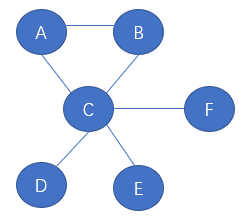
\includegraphics[scale = 0.6]{"C:/Users/Micha/OneDrive - Rensselaer Polytechnic Institute/Graph Theory/pictures/hw3-6.png"}
	\end{figure}
	One match here is edge set $\{AB, CE\}$. The maximum match here has cardinality of 2. We prove this using tutte's condition.
	
	Since there are 6 vertices, $|M_p| = \dfrac{|V(G)|}{2} = 3$. We proceed to prove the graph does not have a perfect match, thus $|M_{max}|<3$. 
	
	If there exists a perfect match for graph G, then $o(G-S) \leq |S|$,  $\forall S \subseteq G$. However, if we remove the vertex c, the odd components are $\{F\},\{D\},\{E\}$. Thus we have $o(G-S) = 3 > 1 >|S|$. Thus the graph does not have a perfect match. Since we have found a match M such that $|M| = 2$ and proved $|M_{max}| < 3$, the match we found above is the maximum match.
	
	\hfill $\blacksquare$
	
	\noindent 7.
	(a).
		Let $S = 4$, then if we remove S, the odd components are $\{1,2,3\}, \{6\}$. Thus $o(G-S) = 2 > 1 >|S|$. Thus Tutte's condition does not hold and perfect match does not exist.
		\begin{figure}[h]
			\hfil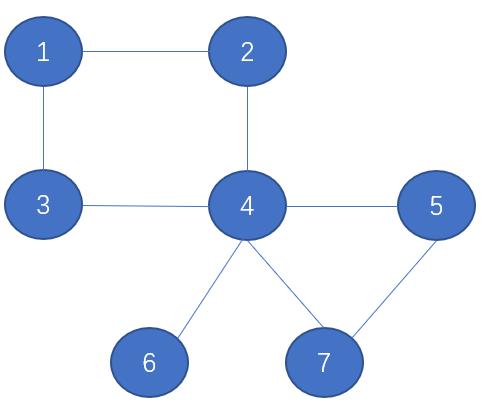
\includegraphics[scale = 0.4]{"C:/Users/Micha/OneDrive - Rensselaer Polytechnic Institute/Graph Theory/pictures/hw3-7-2.png"}\\
		\end{figure}
	
	\newpage
	(b).
		Let us draw the following graph
		
		Note here it is a perfect match since all vertices have been saturated.
	\begin{figure}[h]
		\hfil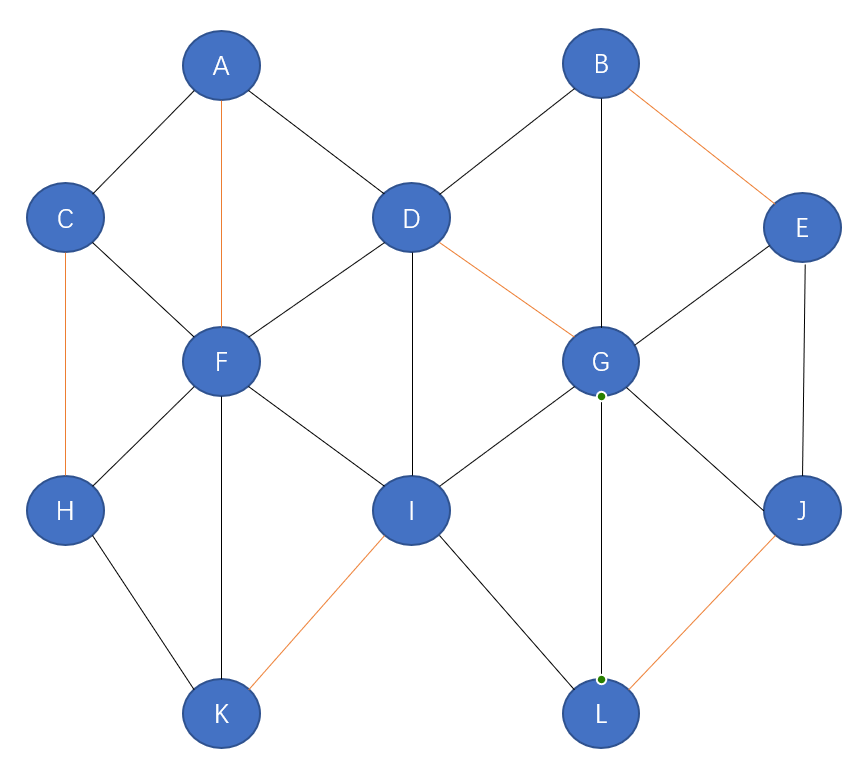
\includegraphics[scale = 0.4]{"C:/Users/Micha/OneDrive - Rensselaer Polytechnic Institute/Graph Theory/pictures/hw3-7-1.png"}\\
	\end{figure}


	
	\noindent 8.
	(a). Vertex cover\\
	\begin{figure}[h]
		\hfil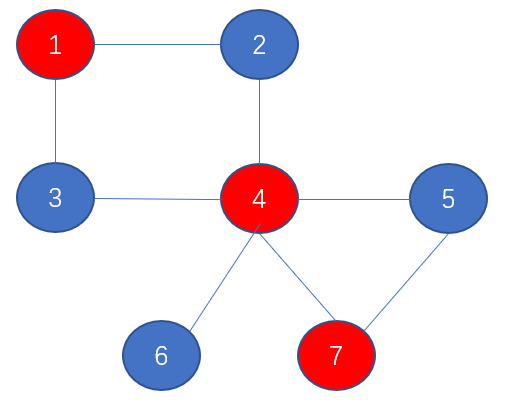
\includegraphics[scale = 0.4]{"C:/Users/Micha/OneDrive - Rensselaer Polytechnic Institute/Graph Theory/pictures/hw3-8-1.png"}\\
	\end{figure}
	\newpage
	(b). Edge cover\\
	\begin{figure}[h]
		\hfil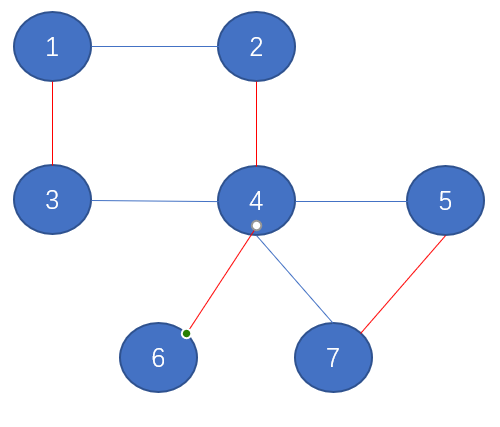
\includegraphics[scale = 0.4]{"C:/Users/Micha/OneDrive - Rensselaer Polytechnic Institute/Graph Theory/pictures/hw3-8-2.png"}\\
	\end{figure}
\end{document}